\documentclass[notitlepage, reprint, nofootinbib]{revtex4-1}
\usepackage[utf8]{inputenc}

% Mathematics and symbols:
\usepackage{amsmath, gensymb, amsthm, physics, mhchem}
% Figures:
\usepackage{tikz, graphicx}
\usepackage[caption=false]{subfig}

% Other:
\usepackage{hyperref}


% Document formatting 
\setlength{\parskip}{1mm}
\setlength{\parindent}{0mm}

% Programming
\definecolor{codebackground}{rgb}{0.9,0.9,0.9}
\usepackage{listings}
\lstset{
	language=python,
	backgroundcolor=\color{codebackground},
	basicstyle=\scriptsize,
	aboveskip={1\baselineskip},
	columns=fixed,
	numbers=left,
	showstringspaces=false, 
	breaklines=true, 
	frame=single,
	showtabs=false,
	showspaces=false,
	keywordstyle=\color[rgb]{0,0,1},
	commentstyle=\color[rgb]{0.133,0.545,0.133}
	}

%\renewcommand{\thesubsubsection}{\alph{subsubsection})}

\hypersetup{
    colorlinks=true,
    linkcolor=blue,
    filecolor=magenta,      
    urlcolor=cyan,
}

\begin{document}
\title{FYS3150 - Project 2}
\author{Frida Larsen}

% Abstract
\begin{abstract}
This report investigates the Jacobi method of solving eigenvalue problems in terms of implementation and accuracy. Although the method is able to reproduce eigenvalues accurately, it only does so under certain conditions. For instance, it must be allowed to perform a high enough number of iterations in order to get an accurate result. The method was also found to be sensitive to the discretization of the problem.
\end{abstract}

\maketitle

\section{Introduction} 
Eigenvalue problems are an important topic of linear algebra and come up in many different settings. Although some eigenvalue problems may be solved analytically, this approach comes with a handful of challenges. The formal method of solving eigenvalue problems, involving determinants and characteristic polynomials,  and the more general method, which relies on different transformations in order to reduce the matrix to diagonal form, are both highly impractical for large matrices.\\[2mm]
The aim of this project is to numerically implement the Jacobi algorithm for solving eigenvalue problems and applying it to the quantum dots system. In order to understand how the algorithm works and how accurate it is, we will continually be comparing it to other methods. Most importantly, we will implement it on the buckling beam system, where the analytical solutions are known, and see how the Jacobi algorithm can best be optimized.\\[2mm]
All relevant code may be found in the GitHub repository 'FYS3150-Computational-Physics'\footnote{\href{GitHub Repository}{https://github.com/fridalarsen/FYS3150-Computational-Physics}} under the Project2 folder. This folder also includes a Figures folder, which holds all the figures presented in this text as well as some additional figures. The program '\texttt{test\_eigenvalue\_problem.py}' contains several different tests for the \texttt{EigenvalueProblem} class which is the main framework of this project. It is located in the '\texttt{eigenvalue\_problem.py}'-program. 
\newpage
\section{Theory}
\subsection{Unitary transformations} 
\subsubsection{Preservation of dot product and orthogonality}\label{dot-orthog}
A unitary transformation of an orthogonal basis $\vb{b}_i$ is given by
\begin{equation}\label{proof1}\vb{a}_i = \vb{U}\vb{b}_i.\end{equation}
Such a transformation preserves the dot product and the orthogonality. To see this, consider first an orthogonal basis of vectors, $\vb{v}_i$, given by
$$\vb{v}_i=\mqty( v_{i1} \\ v_{i2} \\ \vdots \\ v_{in}).$$
For an orthogonal basis 
$$\vb{v}_j^T \vb{v}_i = \delta_{ij}.$$
If this is also true for $\vb{w}$, this basis must also be orthogonal. 
\begin{align*}
	\vb{w}_j^T\vb{w}_i &= (\vb{U}\vb{v}_j)^T (\vb{U}\vb{v}_i) = \vb{U}^T\vb{v}_j^T\vb{U}\vb{v}_i\\ 
	&=\vb{U}^T\vb{U}\vb{v}_j^T\vb{v}_i = \vb{v}_j^T\vb{v}_i \\
	&= \delta_{ij},
\end{align*}
Where we have used that $\vb{U}^T\vb{U}=\vb{I}$ for unitary matrices. And so, $\vb{w}$ is orthogonal and the orthogonality is preserved after the unitary transformation.	 \qed \\[2mm]
If the unitary transformation preserves the dot product we would expect 
$$\vb{w}_j\cdot \vb{w}_i = \vb{v}_j\cdot \vb{v}_i.$$
By using the definition of the dot product, $\vb{a}\cdot\vb{b}=\vb{a}^T\vb{b}$ we get
\begin{align*}
	\vb{w}_j\cdot \vb{w}_i &= \vb{w}_j^T\cdot\vb{w}_i=(\vb{U}\vb{v}_j)^T(\vb{U}\vb{v}_i)\\
	&=\vb{v}_j^T\vb{v}_i=\vb{v}_j\cdot\vb{v}_i,
\end{align*}
where we have used the same property of $\vb{U}$ as explained above. Thus we see that the dot product is also preserved after a unitary transformation. \qed
\subsubsection{Givens rotations}\label{givens}
Consider the unitary transformation of a symmetric matrix $\vb{A}$;
\begin{equation} \label{rotation}\vb{B}=\vb{S}^T\vb{AS},\end{equation}
where $\vb{S}$ is the Givens rotation matrix given by 
\begin{equation}\label{givens_mat} \vb{S}=\mqty( 1&\cdots &0&\cdots &0&\cdots&0\\ \vdots &\ddots & \vdots & &\vdots&&\vdots \\ 0&\cdots&c&\cdots&-s&\cdots&0\\ \vdots &&\vdots&&\vdots&&\vdots\\0&\cdots&s&\cdots&c&\cdots&0\\ \vdots &&\vdots&&\vdots&\ddots&\vdots\\0&\cdots&0&\cdots&0&\cdots&1),\end{equation}
where $s=\sin\theta$, $c=\cos\theta$ and the element $-s$ is located at indices $k$, $l$. In other words, the non-zero elements are given by
\begin{align*}
	s_{kk}&=s_{ll}=\cos\theta=c \\
	s_{kl}&=-s_{lk}=-\sin\theta=-s\\
	s_{ii}&=1,\quad i\neq k, i\neq l.
\end{align*}
After such a transformation, the elements obtained by $\vb{B}$ are 
\begin{align}
	b_{ii}&=a_{ii},\quad i\neq k, i\neq l\nonumber \\
	b_{ik}&=a_{ik}c-a_{il}s,\quad i\neq k, i\neq l\nonumber \\
	b_{il}&=a_{il}c+a_{ik}s,\quad i\neq k, i\neq l\nonumber \\
	b_{kk}&=a_{kk}c^2-2a_{kl}cs+a_{ll}s^2\nonumber \\
	b_{ll}&=a_{ll}c^2+2a_{kl}cs+a_{kk}s^2\nonumber \\
	b_{kl}&=b_{lk}=(a_{kk}-a_{ll})cs+a_{kl}(c^2-s^2).\label{long_thing}
\end{align}

\newpage
\subsection{Buckling Beam Problem}
The vertical displacement, $u(x)$, of a buckling beam of length $L$ obeys 
\begin{equation}\label{bb1}\gamma\dv[2]{u(x)}{x}=-Fu(x),\end{equation}
where $x\in [0,L]$ and $\gamma$ is a constant based on the material properties of the beam. A force $F$ is exerted on the beam at $(L,0)$, pointing towards the origin. The differential equation obeys the Dirichlet conditions $u(0)=u(L)=0$.\\[2mm]
In this project we will assume that $F$ and $L$ are known and attempt to determine $\gamma$ numerically.\\[2mm]
We begin by simplifying the equation above and discretizing it. By setting $\rho = x/L$ and reordering the equation we get 
$$\dv[2]{u(\rho)}{x}=-\frac{FL^2}{\gamma}u(\rho),$$
where $\rho \in [0,1]$. We discretize $\rho$ with $N$ points in the interval $[\rho_0 = 0, \rho_N=1]$. The step-length is then given by 
$$h = \frac{\rho_N-\rho_0}{N},$$
and each point $\rho_i$ can be written as $\rho_i=\rho_0 + ih$, $i=1,2,\dots,N$. The double derivative of a general discretized function $f$ can be approximated by 
\begin{equation}\label{double_deriv}f_i'' \approx \frac{f_{i+1} + f_{i-1}-2f_i}{h^2},\end{equation}
where $h$ is the step-length between each of the points. By this equation we then have 
\begin{equation}\label{bb2}-\frac{u_{i+1}-2u_i+u_{i-1}}{h^2}=\lambda u_i, \end{equation}
where $u_i = u(\rho_i)$ and we have set 
\begin{equation}\label{FL}\lambda=-\frac{FL^2}{\gamma}.\end{equation}
This expression can be then be rewritten as an eigenvalue problem,
\begin{equation}\label{big_boi}\mqty (d&a&0&\dots&0\\a&d&a&\dots&0\\ 0&a&d&\dots&0\\ \vdots&\vdots&\vdots&\vdots&\vdots \\ 0 &\dots&a&d&a) \mqty(u_1\\u_2\\ \vdots\\ u_{N-2}\\u_{N-1})=\lambda \mqty(u_1\\u_2\\ \vdots\\ u_{N-2}\\u_{N-1}),\end{equation}
where $d=2/h^2$ and $a=-1/h^2$. The analytic eigenpairs of this system is given by 
\begin{equation}\label{eigenpairs}\lambda_j = d+2a\cos(\frac{j\pi}{N+1}),\quad j=1,2,\dots,N.\end{equation}
\newpage
\subsection{Quantum dots}
\subsubsection{a single electron}
Consider an electron moving in a 3 dimensional harmonic potential. We assume spherical symmetry. The radial part of the Scrödinger equation for one electron is then given by
$$-\frac{\hbar^2}{2m}\Big(\frac{1}{r^2}\dv{r}r^2\dv{r}-\frac{l (l+1) }{r^2}\Big)R(r)+V(r)R(r)=ER(r),$$
where $V(r)=\frac{1}{2}m\omega^2$ is the harmonic oscillator potential, with $\omega$ being the oscillator frequency. E is the energy of the harmonic oscillator, given by 
$$E_{nl}=\hbar \omega(2n+l+\frac{3}{2}),$$
where $n=0,1,2,\dots$ and $l=0,1,2,\dots$ By using $R(r)=\frac{1}{r}u(r)$ and defining $\rho=\frac{1}{\alpha}r$, where $\alpha$ is some constant of unit length, we get 
$$-\frac{\hbar^2}{2m\alpha^2}\dv[2]{\rho}u(\rho)+\Big(V(\rho)+\frac{l(l+1)}{\rho^2}\frac{\hbar^2}{2m\alpha^2}\Big)u(\rho)=Eu(\rho),$$
with boundary conditions $u(0)=u(\infty)=0$. By setting $l=0$, inserting the potential $V(\rho)=\frac{1}{2}k\alpha^2\rho^2$ and simplifying we get
\begin{equation}\label{simple_tusl}-\dv[2]{\rho}u(\rho)+\rho^2u(\rho)=\lambda u(\rho),\end{equation}
where 
\begin{equation}\alpha=\Big(\frac{\hbar^2}{mk}\Big)^{1/4}\quad\text{and}\quad\lambda=\frac{2m\alpha^2}{\hbar^2}E.\end{equation}
The eigenvalues for $l=0$ are given by
\begin{equation}\label{anal_eig}\lambda = 4n+3,\end{equation}
It remains to discretize the problem in terms of the variable $\rho$. We set $\rho_0=0$, whilst we leave $\rho_N$ to be determined. We cannot set it to $\infty$, but must experiment with large numbers. The step length is then defined as 
$$h=\frac{\rho_N-\rho_0}{N},$$
which means that each point can be found by $\rho_i=\rho_0+ih$, $i=1, 2,\dots,N$. By equation \ref{double_deriv} we get
$$-\frac{u_{i+1}-2u_i+u_{i-1}}{h^2}+V_iu_i=\lambda u_i,$$
where $V_i=\rho_i^2$ is the harmonic oscillator potential. By introducing
$$d_i=\frac{2}{h^2}+V_i\quad\text{and}\quad e_i=-\frac{1}{h^2}$$
we get 
$$d_iu_i+e_iu_{i-1}+e_iu_{i+1}=\lambda u_i.$$
This can in turn be written as an eigenvalue problem:
\begin{equation}\mqty (d_1&e_1&0&\cdots&0&0\\e_1&d_1&e_2&0&\cdots&0\\0&e_2&d_3&\ddots&\vdots&\vdots\\ \vdots&\vdots&\ddots&\ddots&\ddots&0\\0&\cdots&\cdots&\ddots&\ddots&e_{N-2}\\0&0&\cdots&0&e_{N-2}&d_{N-1})\mqty(u_1\\u_2\\ \vdots\\u_{N-1})=\lambda\mqty(u_1\\u_2\\ \vdots\\u_{N-1})\end{equation}
Note that all the non-diagonal elements are equal and that the matrix is symmetric.
\subsubsection{a pair of electrons}
Adding another electron which does not interact with the first electron to the same harmonic oscillator potential results in a different Schrödinger equation, namely 
$$\Big(-\frac{\hbar^2}{2m}\dv[2]{r_1}-\frac{\hbar^2}{2m}\dv[2]{r_2}+\frac{1}{2}kr_1^2+\frac{1}{2}kr_2^2\Big)u(r_1,r_2)=E^{(2)}u/r_1,r_2),$$
where $u(r_1,r_2)$ is the 2-electron wave function and $E^{(2)}$ is the 2-electron energy. By introducing relative coordinates $\vb{r}=\vb{r}_1+\vb{r}_2$ and $\vb{R}=\frac{1}{2}(\vb{r}_1+\vb{r}_2)$ we can write 
$$\Big(\frac{\hbar^2}{m}\dv[2]{r}-\frac{\hbar^2}{4m}\dv[2]{R}+\frac{1}{4}kr^2+kR^2\Big)u(r,R)=E^{(2)}u(r,R),$$
where $u(r,R)=\psi(r)\phi(R)$. We also have $E^{(2)}=E_R+E_r$, where $E_R$ is the center of mass energy and $E_r$ is the relative energy. In reality however, the two electrons interact through the repulsive Coulomb interaction, given by 
$$V(r_1,r_2)=\frac{\beta e^2}{|\vb{r}_1-\vb{r}_2|}=\frac{\beta e^2}{r},$$
where $\beta e^2=1.44$ eVnm. Inserting this into the 2-electron Schrödinger equation, we get 
$$\Big(-\frac{\hbar^2}{m}\dv[2]{r}+\frac{1}{4}kr^2+\frac{\beta e^2}{r}\Big)\psi(r)=E_r\psi(r).$$
By introducing $\rho=\frac{r}{\alpha}$ and simplifying the equation similarly to the one-electron case, we get 
\begin{equation}-\dv[2]{\rho}\psi(\rho)+\omega_r^2\rho^2\psi(\rho)+\frac{1}{\rho}=\lambda\psi(\rho),\end{equation}
where 
\begin{equation}\label{lol}\alpha=\frac{\hbar^2}{m\beta e^2},\quad\omega_r^2=\frac{1}{4}\frac{mk\alpha^4}{\hbar^2}\quad \text{and}\quad \lambda=\frac{m\alpha^2}{\hbar^2}E.\end{equation}
Here, $\omega_r$ is a parameter reflecting the strength of the oscillator potential. 
\newpage
\section{Method}
\subsection{The Jacobi Method}
The main idea behind the Jacobi method is to perform a series of Givens rotations as described in section \ref{givens} in order to turn a symmetric matrix $\vb{A}$ into a diagonal matrix such that the eigenvalues can be read off the diagonal. In order to acheive this, we must choose $k$, $l$ and $\theta$ for each rotation such that the diagonal elements of the transformed matrix, $\vb{B}$, approach zero. When this happens, $b_{kl}=b_{lk}=0$. From the expressions for the diagonal elements in equation (\ref{long_thing}) we get 
$$b_{kl}=a_{kl}(c^2-s^2)+(a_{kl}-a_{ll})cs=0\implies c=1, s=0.$$ 
By defining 
$$\tan\theta=t=\frac{s}{c}\quad\text{and}\quad \cot 2\theta=\tau=\frac{a_{ll}-a_{kk}}{2a_{kl}}$$
we can write
$$t^2+2t\tau-1=0\implies t=-\tau \pm \sqrt{1+\tau^2}.$$
It then follows that 
$$c=\frac{1}{\sqrt{1+t^2}}\quad \text{and}\quad s=tc.$$
We always wish to minimize the largest of the elements of $\vb{A}$, and the indices $k$ and $l$ must be chosen with this in mind. \\[2mm]
Considering the fact that we are working numerically, it is worth noting that the diagonal elements might take a very very large number of rotations to become precisely 0. In order to circumvent this, we set the tolerance of the algorithm to $10^{-12}$.\\[2mm]
As the Givens rotation is a unitary transformation, we know from section \ref{dot-orthog} that the eigenvectors of the final matrix have preserved dot product and orthogonality. We can use this in order to test the validity of the program\footnote{See the test functions mentioned in the introduction.}.   
\subsection{NumPy and Armadillo libraries}
In order to get a better understanding of how the Jacobi method performs, we will use the NumPy \texttt{linalg} library\cite{NumPy_linalg} and Armadillo functions\cite{Arma1}\cite{Arma2} for computing eigenvectors as a comparison to both the analytical values and the Jacobi method values. 






\section{Results}
Figure \ref{eigenvectors_bb} shows the three first eigenvectors of the buckling beam problem as calculated with Armadillo and the Jacobi method. For the latter, the maximum number of iterations was $10^3$. Figure \ref{relative_max_error} shows the relative maximum error of the Armadillo and Jacobi algorithm in calculating the eigenvalues as compared to the analytic eigenvalues. The Jacobi algorithm is plotted as a function of the number of maximum iterations allowed. Table \ref{lambdas} shows the $\lambda$s obtained with the different methods through equation \ref{FL} with $F=L=1$. The number of maximum rotations used for the Jacobi algorithm was $10^3$. \\[2mm]
Figure \ref{eigvec_qdots1} shows a plot of the three first eigenvectors of an electron in a 3 dimensional harmonic oscillator potential as calculated by the Jacobi method. The corresponding eigenvalues are indicated in the top-right corner. Figure \ref{qdots2} shows the error of the eigenvalues found using the Jacobi method as compared to the expected eigenvalues from equation \ref{anal_eig}. The error is plotted as a function of both $N$ and $\rho_{max}$.\\[2mm]
Table \ref{lambda_table} shows the first 5 eigenvalues of two electrons in a 3 dimensional harmonic oscillator potential for different values of $\omega_r$. The values were computed using the Jacobi algorithm with a maximum of $10^4$ rotations. Figure \ref{2dots_vector} shows a plot of the three first eigenvectors and their corresponding eigenvalues in the $\omega_r=0.01$ case. The eigenvector plots for the remaining $\omega_r$s may be found in the Figures folder as discussed in the introduction.
\begin{figure}[h!]
	\centering
	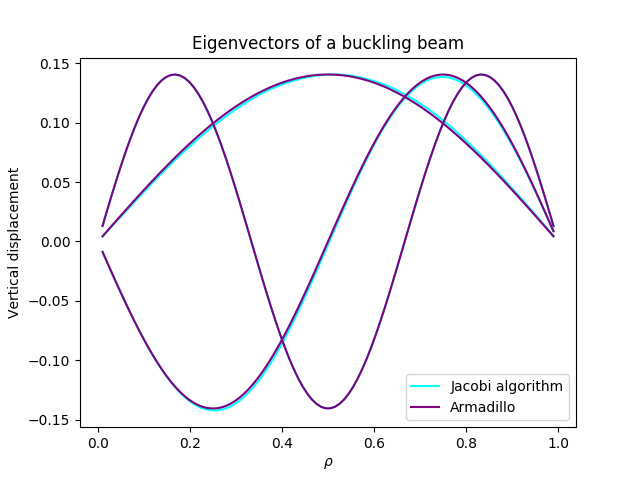
\includegraphics[width=0.5\textwidth]{../Figures/eigenvectors_buckling_beam.png}
	\caption{Eigenvectors of a buckling beam calculated with Armadillo and the Jacobi method.}
	\label{eigenvectors_bb}
\end{figure}
\begin{figure}[h!]
	\centering
	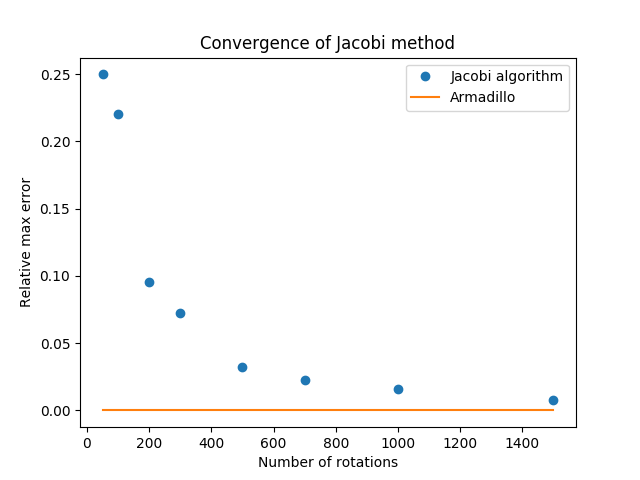
\includegraphics[width=0.5\textwidth]{../Figures/relative_max_error.png}
	\caption{Relative max error of Jacobi algorithm and Armadillo for different number of maximum rotations.}
	\label{relative_max_error}
\end{figure}
\begin{table}[h!]
\centering
\begin{tabular}{|c|c|}
\hline
Method & $\lambda$ obtained \\ \hline
NumPy & -0.101329 \\ \hline
Armadillo & -0.101329 \\ \hline
Jacobi (Python) & -0.101223 \\ \hline
Jacobi (C++) & -0.101223 \\ \hline
\end{tabular}
\caption{Lambda-values obtained using 4 different methods. The Jacobi methods had max rotations set to $10^3$.}
\label{lambdas}
\end{table}
\begin{figure}[h!]
	\centering
	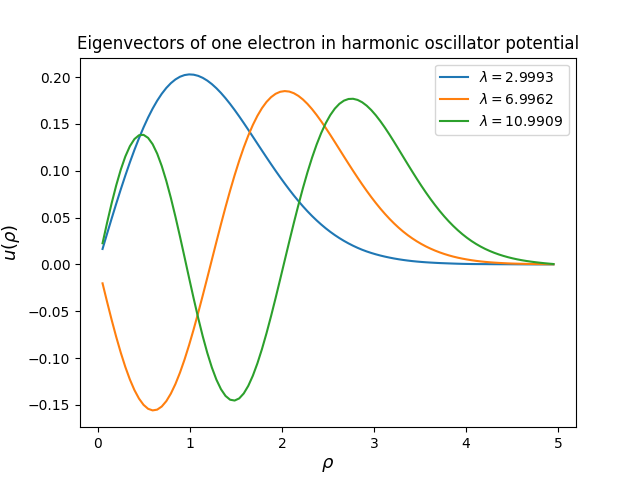
\includegraphics[width=0.5\textwidth]{../Figures/eigvec_qdots1.png}
	\caption{Eigenvectors of an electron in a 3D harmonic oscillator potential.}
	\label{eigvec_qdots1}
\end{figure}
\begin{figure}[h!]
	\centering
	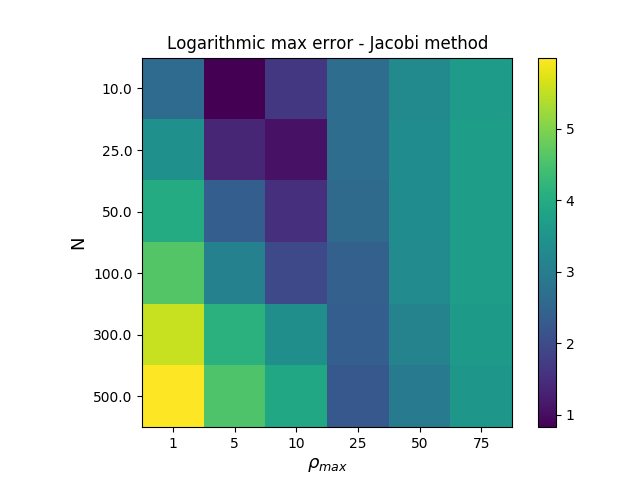
\includegraphics[width=0.5\textwidth]{../Figures/error_colorbar_qdots2.png}
	\caption{Colorbar plot of the error of eigenvalues found using the Jacobi method as a function of $N$ and $\rho_{max}$.}
	\label{qdots2}
\end{figure}
\newpage
\begin{table}[h!]
\centering
\begin{tabular}{|c|c|c|c|c|c|}
\hline
$\omega_r$ & \multicolumn{5}{l|}{eigenvalues} \\ \hline
0.01 & 0.8411 & 2.1730 & 4.2348 & 7.0556 & 10.6444 \\ \hline
0.5 & 2.2309 & 4.1683 & 6.3832 & 9.1982 & 12.7672 \\ \hline
1.0 & 4.0572 & 7.9060 & 11.8105 & 15.7476 & 19.7730 \\ \hline
5.0 & 17.4286 & 36.9772 & 56.6229 & 76.2758 & 95.9041 \\ \hline
\end{tabular}
\caption{First five computed eigenvalues using the Jacobi algorithm with different values of $\omega_r$.}
\label{lambda_table}
\end{table}
\begin{figure}[h!]
	\centering
	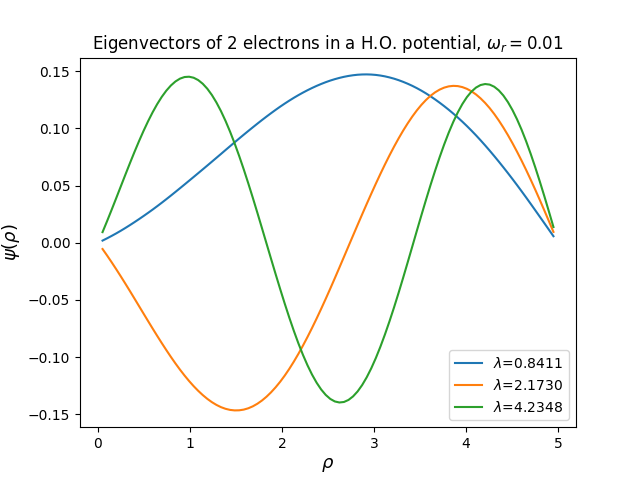
\includegraphics[width=0.5\textwidth]{../Figures/eigvec_qdots2_0.png}
	\caption{The first three eigenvectors of two electrons in a harmonic oscillator potential and their corresponding eigenvalues for $\omega_r=0.01$.}
	\label{2dots_vector}
\end{figure}
\clearpage
\section{Discussion}
From figure \ref{relative_max_error} we see that for the buckling beam the Jacobi method converges to the analytical solution for a larger number of iterations allowed. For certain problems, this would not be the case. It depends on how the original matrix looks. This is a downside to the Jacobi method as it is hard to predict whether or not the matrix will become diagonal quickly or if at all.\\[2mm]
From the same plot we also see that Armadillo did a very good job of finding the correct eigenvalues. Table \ref{lambdas} tells us that the Armadillo and NumPy methods behaved similarly. The same was true for the two Jacobi methods, although they were written in different languages. This is to be expected as the algorithm is the same. However, we did notice that the C++ version took significantly less time to run although it took a while longer to write. \\[2mm]
From figure \ref{qdots2} we see that there seems to be a diagonal line of stability going left to right where the error is smaller. It seems logical that a huge $\rho_{max}$ should give a better result as the framework requires $\rho_{max}=\infty$, but this is not always the case. Only as $N$ increases significantly in size does a large $\rho_{max}$ give better results. \\[2mm]
From table \ref{lambda_table} we see that for the 2 electrons in the harmonic oscillator potential, a larger $\omega_r$ results in a larger $\lambda$. In turn, a larger $\lambda$ indicates a larger energy by equation \ref{lol}. $\omega_r$ is a measure of the oscillator strength, and it makes sense that a larger oscillator strength would result in a larger energy. 

\section{Conclusion}
The aim of this project was to implement the Jacobi method for solving eigenvalue problems and exploring its uses and limitations. Overall, we found that the Jacobi algorithm is heavily dependent on the number of maximum iterations it is allowed to perform. The more the better seems to be the case for larger problems. We also found that the algorithm is susceptible to errors related to how the problem is discretized. 


\onecolumngrid
\bibliographystyle{unsrtnat}
\bibliography{references.bib}

\end{document}